\documentclass[german, % Standardmäßig deutsche Eigenarten, englisch -> english
parskip=full, % Absätze durch Leerzeile trennen
bibliography=totoc, % Literatur im Inhaltsverzeichnis
%draft, % TODO: Entwurfsmodus -> entfernen für endgültige Version
]{scrartcl}
\usepackage{ifluatex} % zum Testen, ob LuaTeX verwendet wird
\ifluatex
\usepackage{fontspec} % Laden von Schriften
\setmainfont[Mapping=tex-text]{Linux Libertine O}  % Mapping ermöglicht die Verwendung z.B. von --
\setsansfont[Mapping=tex-text]{Linux Biolinum O}
\usepackage{polyglossia}  % Sprachpaket
\setdefaultlanguage[spelling=new,babelshorthands=true]{german}  % Neue Rechtschreibung und Abkürzungen
\else % kein LuaTeX
\usepackage[utf8]{inputenc} % Kodierung der Datei
\usepackage[T1]{fontenc} % Vollen Umfang der Schriftzeichen
\usepackage{lmodern}
\usepackage[ngerman]{babel} % Sprache auf Deutsch (neue Rechtschreibung)
%\usepackage{libertine} % Schriftart Linux Libertine/Biolinum verwenden
\fi

% Mathematik und Größen
\usepackage{amsmath}
\ifluatex
\usepackage{unicode-math}
\fi
\usepackage[locale=DE, % deutsche Eigenarten, englisch -> US
separate-uncertainty, % Unsicherheiten seperat
]{siunitx}
\usepackage{physics} % Erstellung von Gleichungen vereinfachen

% Bilder einbinden
\usepackage{graphicx}
\usepackage{float}
\usepackage{caption}
%\graphicspath{{bilder/}} % TODO: Pfad unter dem die Bilder gesucht werden

% Gestaltung
\usepackage{microtype}  % Mikrotypographie
\usepackage{booktabs}  %schönere Tabellen
\usepackage{multirow}
%\usepackage[toc]{multitoc}  %mehrspaltiges Inhaltsverzeichnis
\usepackage{csquotes} % Anführungszeichen mit \enquote
\usepackage{subcaption}  % Unterabbildungen a,b,c,…
\usepackage{enumitem}  % Listen anpassen
\setlist{itemsep=-10pt}
\usepackage{scrpage2}  % Manipulation des Seitenstils
% Kopf-/Fußzeilen
\pagestyle{scrheadings}
\clearscrheadings
\automark{section}
\ofoot{\pagemark}
\ihead{\headmark}
\setheadsepline{.5pt}

\usepackage[colorlinks=true]{hyperref}  % Links und weitere PDF-Features

\makeatletter 
\renewcommand\subsection{\@startsection 
   {subsection}{2}{0mm}%      % name, ebene, einzug 
   {0.5\baselineskip}%            % vor-abstand 
   {0.3\baselineskip}%            % nach-abstand 
   {\bfseries\sffamily\large}%           % layout 
   } 
\makeatother 

% TODO: Titel und Autor, … festlegen
\newcommand*{\titel}{Gammaspektroskopie}
\newcommand*{\autor}{Maximilian Obst, Thomas Adlmaier}
\newcommand*{\abk}{GA}
\newcommand*{\betreuer}{Dr. Alexander Domula}
\newcommand*{\messung}{16.12.2016}
\newcommand*{\ort}{Technische Universität Dresden, IKTP}

\hypersetup{pdfauthor={\autor}, pdftitle={\titel}} % PDF-Metadaten

\titlehead{F-Praktikum \abk \hfill TU Dresden}
\subject{Versuchsprotokoll}
\title{\titel}
\author{\autor}
\date{\begin{tabular}{ll}
Protokoll: & \today\\
Messung: & \messung\\
Ort: & \ort\\
Betreuer: & \betreuer\end{tabular}}

%----------------
\begin{document}
\begin{titlepage}
\maketitle

\begin{figure}[hb] 
  \centering
     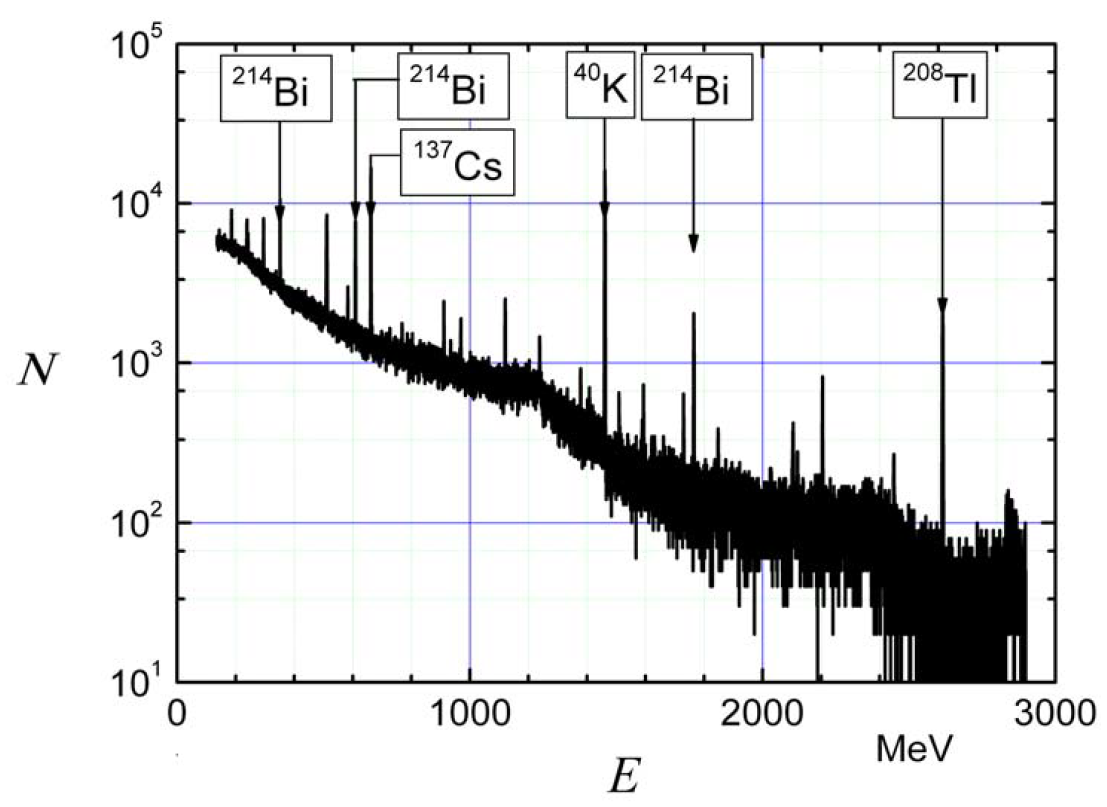
\includegraphics[width=0.8\textwidth]{untergrund}
  \caption{Typisches Untergrund-Gammaspektrum. Die erkennbaren Peaks wurden den zugehörigen Radionukliden zugeordnet}
  \label{fig:untergrund}
\end{figure}

\end{titlepage}

\tableofcontents
\pagebreak

%------------------------
\section{Physikalische Grundlagen}

Die Gammaspektroskopie befasst sich mit dem Nachweis sowie der quantitativen Untersuchung von Gammastrahlen und -strahlern. In diesem Versuch geht es darum, die Grundlagen der Gammaspektroskopie zu lernen. Dafür werden mit zwei unterschiedlichen Detektoren verschiedene radioaktive Materialien untersucht. 

\subsection{Gammastrahlung}

Atome bilden die Grundlage der Materie. Sie sind jedoch nicht immer stabil: Entweder durch ihren eigenen Aufbau bedingt oder durch Störungen von außerhalb können Atomkerne zerfallen. Dabei entstehen unterschiedliche Teilchen, die als Strahlung gelten. Es gibt drei Arten von Strahlung:
\begin{itemize}
\item \textbf{Alpha-Strahlung:} Hier werden beim Zerfall des Atomkerns He\textsuperscript{2+}-Kerne freigesetzt. Diese sind sehr schwer und können daher schwere Schäden in ihrer Umgebung anrichten. Allerdings fliegen diese Teilchen nicht sehr weit und können gut abgeschirmt werden.
\begin{align}
{}^A_Z\mathrm{X} \to {}^{A-2}_{Z-2}\mathrm{Y} + {}^2_2\mathrm{He} \label{for:alpha}
\end{align}
\item \textbf{Beta-Strahlung:} Bei dieser Strahlungsart wandelt sich ein Neutron in ein Proton oder umgekehrt. Die entstehenden Elektronen oder Positronen fliegen weiter als Alpha-Teilchen, haben aber auch eine verringerte schädingende Wirkung.
\begin{align}
{}^A_Z\mathrm{X} \to {}^{A}_{Z+1}\mathrm{Y} + e^- + \bar \nu_e \label{for:beta-} \\ 
{}^A_Z\mathrm{X} \to {}^{A}_{Z-1}\mathrm{Y} + e^+ + \nu_e \label{for:beta+}
\end{align}
\item \textbf{Gamma-Strahlung:} Diese Strahlung führt nicht zu einer Veränderung des Atomkerns sondern bringt diesen nur von einem angeregten Zustand zurück in den Grundzustand. Dabei werden hochenergetische Photonen ausgesendet, die nur schwach schädigend wirken, aber eine hohe Reichweite haben und kaum abzuschirmen sind. Durch diese Eigenschaften sowie die Proportionalität der messbaren Photonenenergie zur Zerfallsenergie eignet sich Gamma-Strahlung besonders gut zur Untersuchung radioaktiver Stoffe und Zerfälle.
\begin{align}
{}^A_Z\mathrm{X*} \to {}^{A}_{Z}\mathrm{X} + \gamma \label{for:gamma}
\end{align}
\end{itemize}

\subsection{Gamma-Detektoren}

Photonen wechselwirken nur schwach mit Materie. Um sie dennoch nachzuweisen, wird ihre ionisierende Wirkung genutzt. Dabei werden drei auftretende, messbare Effekte unterschieden:
\begin{itemize}
\item \textbf{Photoeffekt: }Photonen niedriger Energie können bei Kollisionen mit den Elektronen der Atomhülle ihre gesamte Energie an die Elektronen übertragen. Ist die übertragene Energie groß genug, löst sich das Elektron aus seiner Bindung mit dem Atomkern und ein Elektron-Ion-Paar entsteht. 
\item \textbf{Inkohärente Streuung: }Bei höheren Photonenenergien wird nicht mehr die gesamte Energie des Photons bei Stößen mit den Elektronen der Atomhülle übertragen, sondern nur ein Teil. Beide Kollisionsteilnehmer ändern ihre Richtung.
\item \textbf{Paarbildung: }Noch höhere Photonenenergien können Stöße mit den Elektronen der Atomhülle zur Paarbildung führen: Das Photon erzeugt ein Positron und ein Elektron. Die übrige Energie erhalten die erzeugten Ladungsträger als kinetische Energie.
\end{itemize}
Dabei tragen die entstehenden Ladungsträger bei Photoeffekt und Paarbildung die gesamte Energie des Photons. Bild \ref{fig:gammaww} zeigt die Energiebereiche, in denen die jeweiligen Prozesse stattfinden, sowie deren Wahrscheinlichkeit. Diese ist von der Ordnungszahl $Z$, der Massenzahl $A$, der Dichte $\rho$ und der Photonenenergie $E$ abhängig. 

\begin{figure}[ht] 
  \centering
     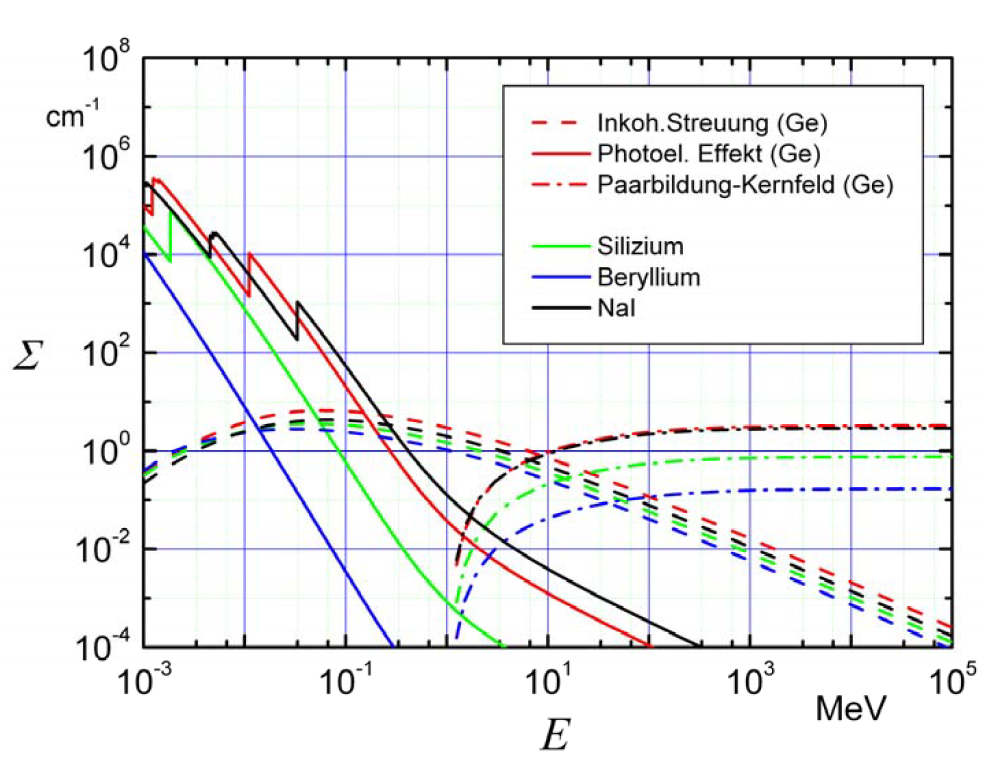
\includegraphics[width=0.9\textwidth]{gammaww}
  \caption{Wechselwirkungsquerschnitte für verschiedene Effekte der Photon-Atom-Wechselwirkung. Zur Verdeutlichung der Abhängigkeit der Reaktionen von der Ordnungszahl $Z$ der Atome sind die Querschnitte von Reaktionen mit Silizium, Beryllium und Germanium dargestellt}
  \label{fig:gammaww}
\end{figure}

Zur Messung der Effekte gibt es zwei Möglichkeiten:
\begin{itemize}
\item In einem ladungsträgerverarmten Material erzeugt die Gamma-Strahlung Ladungsträger. Durch ein angelegtes elektrisches Feld werden diese beschleunigt und die entstehende Spannung gemessen. Zur Verbesserung der Messbarkeit wird entweder Ladungsträgervervielfachung durch Sekundärionisation oder eine Verstärkung der empfangenen Signale genutzt.
\item In einer photoaktiven Schicht erzeugen die einfallenden Photonen Photonen im ultravioletten Frequenzbereich. Diese Photonen erzeugen in einer Photokathode Elektronen, die in einem Photo-Sekundär-Elektronen-Vervielfacher vervielfacht werden, bis ein gut messbares Signal entsteht (siehe Bild \ref{fig:szintillator}).
\end{itemize}

\begin{figure}[ht] 
  \centering
     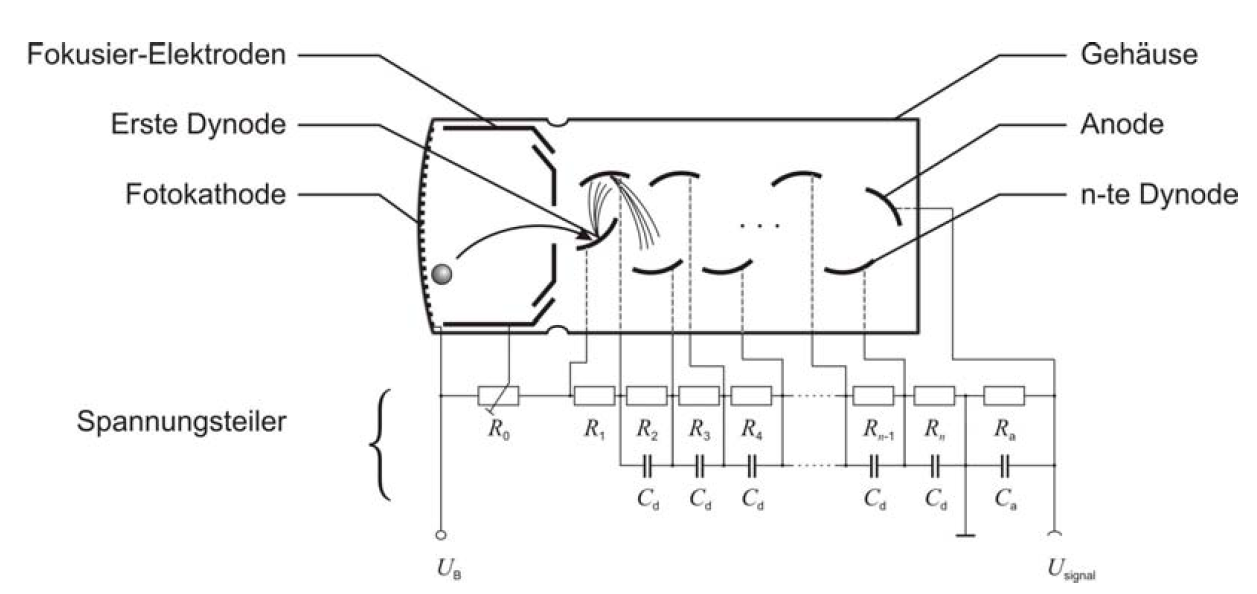
\includegraphics[width=0.9\textwidth]{Szintillatoraufbau}
  \caption{Aufbau und Funktionsweise eines Photo-Sekundär-Elektronen-Vervielfachers, wie er in Szintillator-Detektoren seinen Einsatz findet}
  \label{fig:gammaww}
\end{figure}

Im Versuch wird als Szintillator ein NaI(Tl)-Detektor (Natriumiodid als szintillierendes Material) und ein High-Puritiy-Germanium-Detektor (kurz HP-Ge-Detektor) verwendet. Der HP-Ge-Detektor verwendet als ladungsträgerverarmtes Material eine Halbleiter-Diode. Diese wird hierbei in Sperrrichtung betrieben. Hochreines Germanium eignet sich dabei bestens als Halbleitermaterial: Die Ladungsträgermobilität ist eher mittelmäßig, die nötige Energie zur Erzeugung eines Elektron-Loch-Paares mit \SI{2.95}{\electronvolt} jedoch sehr klein. Des Weiteren bildet eine Germanium-p-i-n-Diode ein besonders großes aktives Volumen aus. Außerdem haben alle anderen Materialien, die für eine solche Diode nutzbar währen, eine kleinere Ordnungszahl als Germanium ($Z$ = 32) und damit einen kleineren Wechselwirkungsquerschnitt mit Photonen. Der Aufbau sowie die Funktionsweise eines HP-Ge-Detektors kann in Bild \ref{fig:hpged} gesehen werden.

\begin{figure}[ht] 
  \centering
     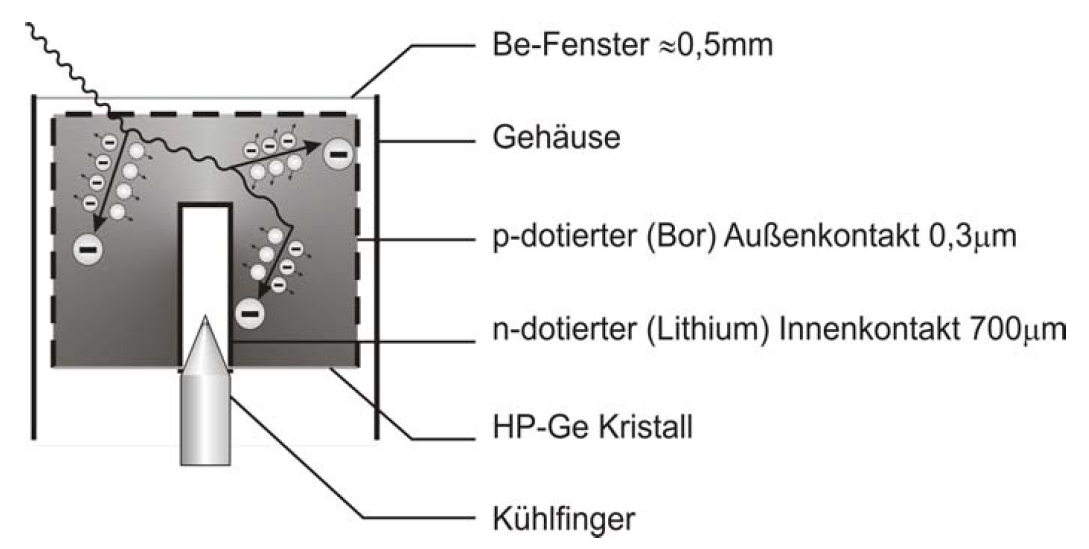
\includegraphics[width=0.9\textwidth]{HPGeDetektor}
  \caption{Aufbau und Funktionsweise eines HP-Ge-Detektors}
  \label{fig:hpged}
\end{figure}

HP-Ge-Detektoren haben ein weitaus höheres Energieauflösungsvermögen als Szintillatoren, daher sind Peaks in den Ereigniszahlen besser voneinander unterscheidbar und besser zuzuordnen. Demgegenüber sind Szintillatoren jedoch robuster und benötigen keine Kühlung, was sie transportabler macht. Außerdem sind Szintillatoren günstiger als HP-Ge-Detektoren.

\subsection{Spektrenanalyse}

Gammaspektren zeigen einen typischen Aufbau mit üblicherweise drei Peaks, von denen die ersten beiden zum Compton-Spektrum gehören, zu dem die meisten der gemessenen Ereignisse gehören:
\begin{itemize}
\item \textbf{Rückstreupeak: }Dieser Peak entsteht, wenn das Photon schon einen Teil seiner Energie außerhalb des aktiven Materials deponiert hat. Wenn das Photon nun seine restliche Energie über inkohärente Streuung an Elektronen im aktiven Material abgibt, wird die maximale Energie bei Rückstreuung übertragen ($\theta$ = \SI{180}{\degree}). Daher stammt der Name dieses Peaks. Die übertragene Energie kann mit Formel \ref{for:rueckstreu} berechnet werden. Die maximal mögliche Energie dieses Peaks liegt bei \SI{255.5}{\kilo\electronvolt}.
\begin{align}
E = E' \frac{1}{1 + \frac{E'}{m_e c^2} (1 - \cos (\theta))} \label{for:rueckstreu}
\end{align}
\item \textbf{Compton-Kante: }Wenn das Photon erst einen Teil seiner Energie im aktiven Material abgibt und den Rest danach außerhalb, entsteht dieser Peak. Dabei wird durch inkohärente Streuung ein Elektron aus der Atomhülle gelöst. Die deponierte Energie kann mit Formel \ref{for:comptonk} berechnet werden.
\begin{align}
E = E' (1 - \frac{1}{1 + \frac{E'}{m_e c^2} (1 - \cos (\theta))}) \label{for:comptonk}
\end{align}
\item \textbf{Vollenergiepeak: }Dieser Peak, der üblicherweise der höchste des Spektrums und der am leichtesten erkennbare ist, entsteht, wenn die gesamte Energie eines Photons im aktiven Material abgegeben wurde. Der Vollenergiepeak wird zur Bestimmung der strahlenden Materialien genutzt.
\end{itemize}
In Bild \ref{fig:gammaspektrum} können die einzelnen Peaks anhand des Spektrums einer \textsuperscript{137}Cs-Gammaquelle nachvollzogen werden. In diesem Bild kann auch eine Ereigniszahl vor dem Compton-Spektrum festgestellt werden. Dies ist ein Teil des Messuntergrundes, der durch Höhenstrahlung und die natürliche Radioaktivität der Umgebung bedingt ist. Die Untergrundstrahlung muss bei jeder Messung berücksichtigt werden und führt im Zweifel dazu, dass einzelne Peaks nicht mehr sichtbar sind, weil sie darin "`verschwinden"'. Ein typisches Bild eines Untergrundspektrums kann in Bild \ref{fig:untergrund} gesehen werden.

\begin{figure}[ht] 
  \centering
     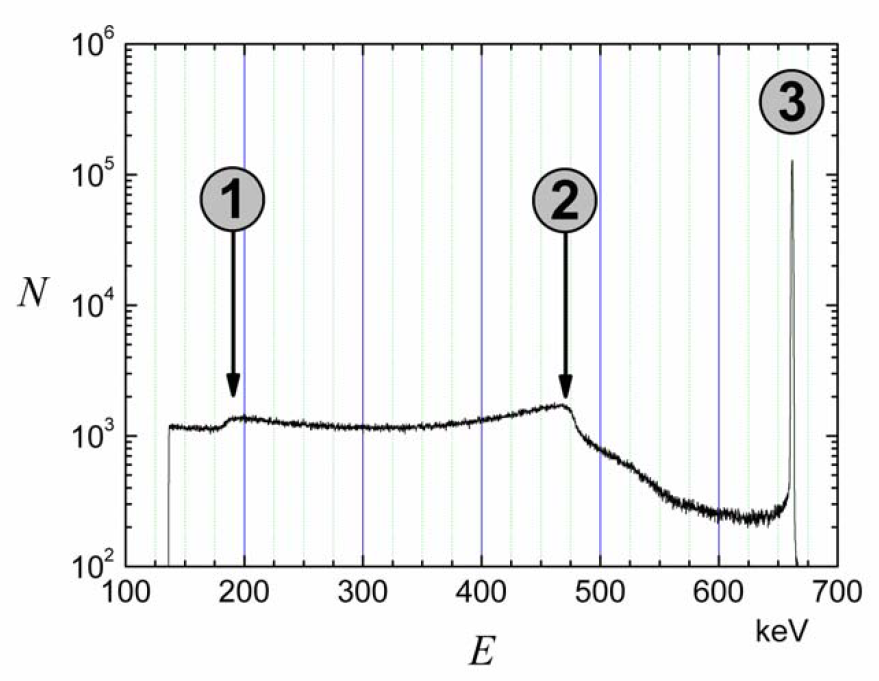
\includegraphics[width=0.9\textwidth]{gammaspektrum}
  \caption{Gammaspektrum einer \textsuperscript{137}Cs-Quelle. Peak 1 und 2 bilden das Compton-Spektrum, wobei Peak 1 der Rückstreupeak und Peak 2 die Compton-Kante ist. Peak 3 ist der Vollenergiepeak}
  \label{fig:gammaspektrum}
\end{figure}

\subsection{Aktivität}

Die Aktivität einer Probe beschreibt die Anzahl von Ereignissen, die von der Probe stammen, über einen festen Zeitraum. Die Einheit ist Becquerel (kurz Bq, [Bq] = N/s). Um die Aktivität einer Probe zu bestimmen, müssen verschiedene Arbeitsschritte durchgeführt werden:
\begin{enumerate}
\item \textbf{Kalibrierung: }Zunächst muss das Spektrum kalibriert werden. Als erstes wird dabei die Energiekalibrierung durchgeführt. Dafür wird das Spektrum einer Probe mit einem bekannten Radionuklid aufgenommen und die sichtbaren Peaks Peaks bekannter Energie zugeordnet. So wird klar, welcher Kanal zu welcher Energie gehört. Als nächstes muss das Vollenergieansprechvermögen des Detektors bestimmt werden.
\item \textbf{Untergrundmessung: }Um die Aktivität zu bestimmen, dürfen nur die Ereigniszahlen der Probe berücksichtigt werden. Daher wird eine Messung ohne Probe gemacht, um später den Untergrund von der Messung abziehen zu können.
\item \textbf{Messung der Probe: }Der nächste Schritt ist der letzte Schritt experimenteller Art. Nun wird die untersuchte Probe gemessen.
\item \textbf{Analyse: }Im letzten Schritt wird mithilfe der Messdaten die Aktivität bestimmt. Dabei wird zum einen die Messung mithilfe der Untergrundmessung korrigiert. Zum anderen werden Koinzidenzereignisse, bei denen zwei oder mehr Photonen innerhalb einer Totzeit ihre Energie im Detektor deponieren, auf die Anzahl ihrer Photonen untersucht und diese Photonen getrennt berücksichtigt. Außerdem wird die Messung um ihre geometrischen Faktoren korrigiert, z.B. werden die Ereigniszahlen auf den gesamten Raumwinkel hochgerechnet.
\end{enumerate}

\subsection{Vollenergieansprechvermögen}

Das absolute Vollenergieansprechvermögen (VEAV) $\epsilon$ beschreibt Abweichung der gemessenen Ereignisse von der tatsächlichen Zahl der Ereignisse. Es ist einer der Gütegrade eines Gammadetektors: Je höher das VEAV, desto besser kann gemessen werden. Im Unterschied zum totalen Ansprechvermögen (TAV), werden hierbei nur die Ereignisse im Vollenergiepeak gezählt. 
\begin{align}
\epsilon (E_{\gamma}) = \frac{registrierte Ereignisse}{mögliche Ereignisse} = \frac{N (\gamma_i)}{A t_L \nu_{\gamma_i}} \label{for:veav}
\end{align}
Das VEAV wird mithilfe einer Kalibrierprobe bestimmt. Es unterscheidet sich je nach Energie der detektierten Photonen: Da nahezu alle Materialien bei niedrigerer Energie einen höheren Wechselwirkungsquerschnitt mit Photonen haben, steigt das VEAV, je niedriger die Photonenenergie ist. Bei sehr niedrigen Energien jedoch gelangt nur noch ein kleiner Teil der Photonen überhaupt in das aktive Volumen, das VEAV sinkt rapide ab.

\section{Durchführung}

Mithilfe eines High-Purity-Germanium-Detektors (HP-Ge-Detektor) und eines Szintillators werden die Spektren von Cobalt, Caesium, Americium, Barium und Europium untersucht. Die Ergebnisse des Germanium-Detektors und des Szintillators werden bezüglich ihrer Vollenergie-Ansprechvermögen und ihres Auflösungsvermögens verglichen. Als letztes wird eine unbekannte Probe mithilfe des HP-Ge-Detektors auf ihre Ausgangsstoffe untersucht. 

\section{Analyse}



\section{Diskussion}



\subsection{Fazit}



%------------------------

\begin{thebibliography}{9}

\bibitem{eisen}
  https://de.wikipedia.org/wiki/Eisen
	19.12.2016
	17:50 Uhr

\end{thebibliography}

\section{Anhang: Arbeitsplatzprotokoll}



\end{document}
